\documentclass[border=10pt]{standalone}

\usepackage{tikz}
\usepackage{tikzsymbols}
\usetikzlibrary{calc,patterns,shapes.geometric}

\def\centerarc[#1](#2)(#3:#4:#5){\draw[#1] ($(#2)+({#5*cos(#3)},{#5*sin(#3)})$) arc (#3:#4:#5);}

\begin{document}
	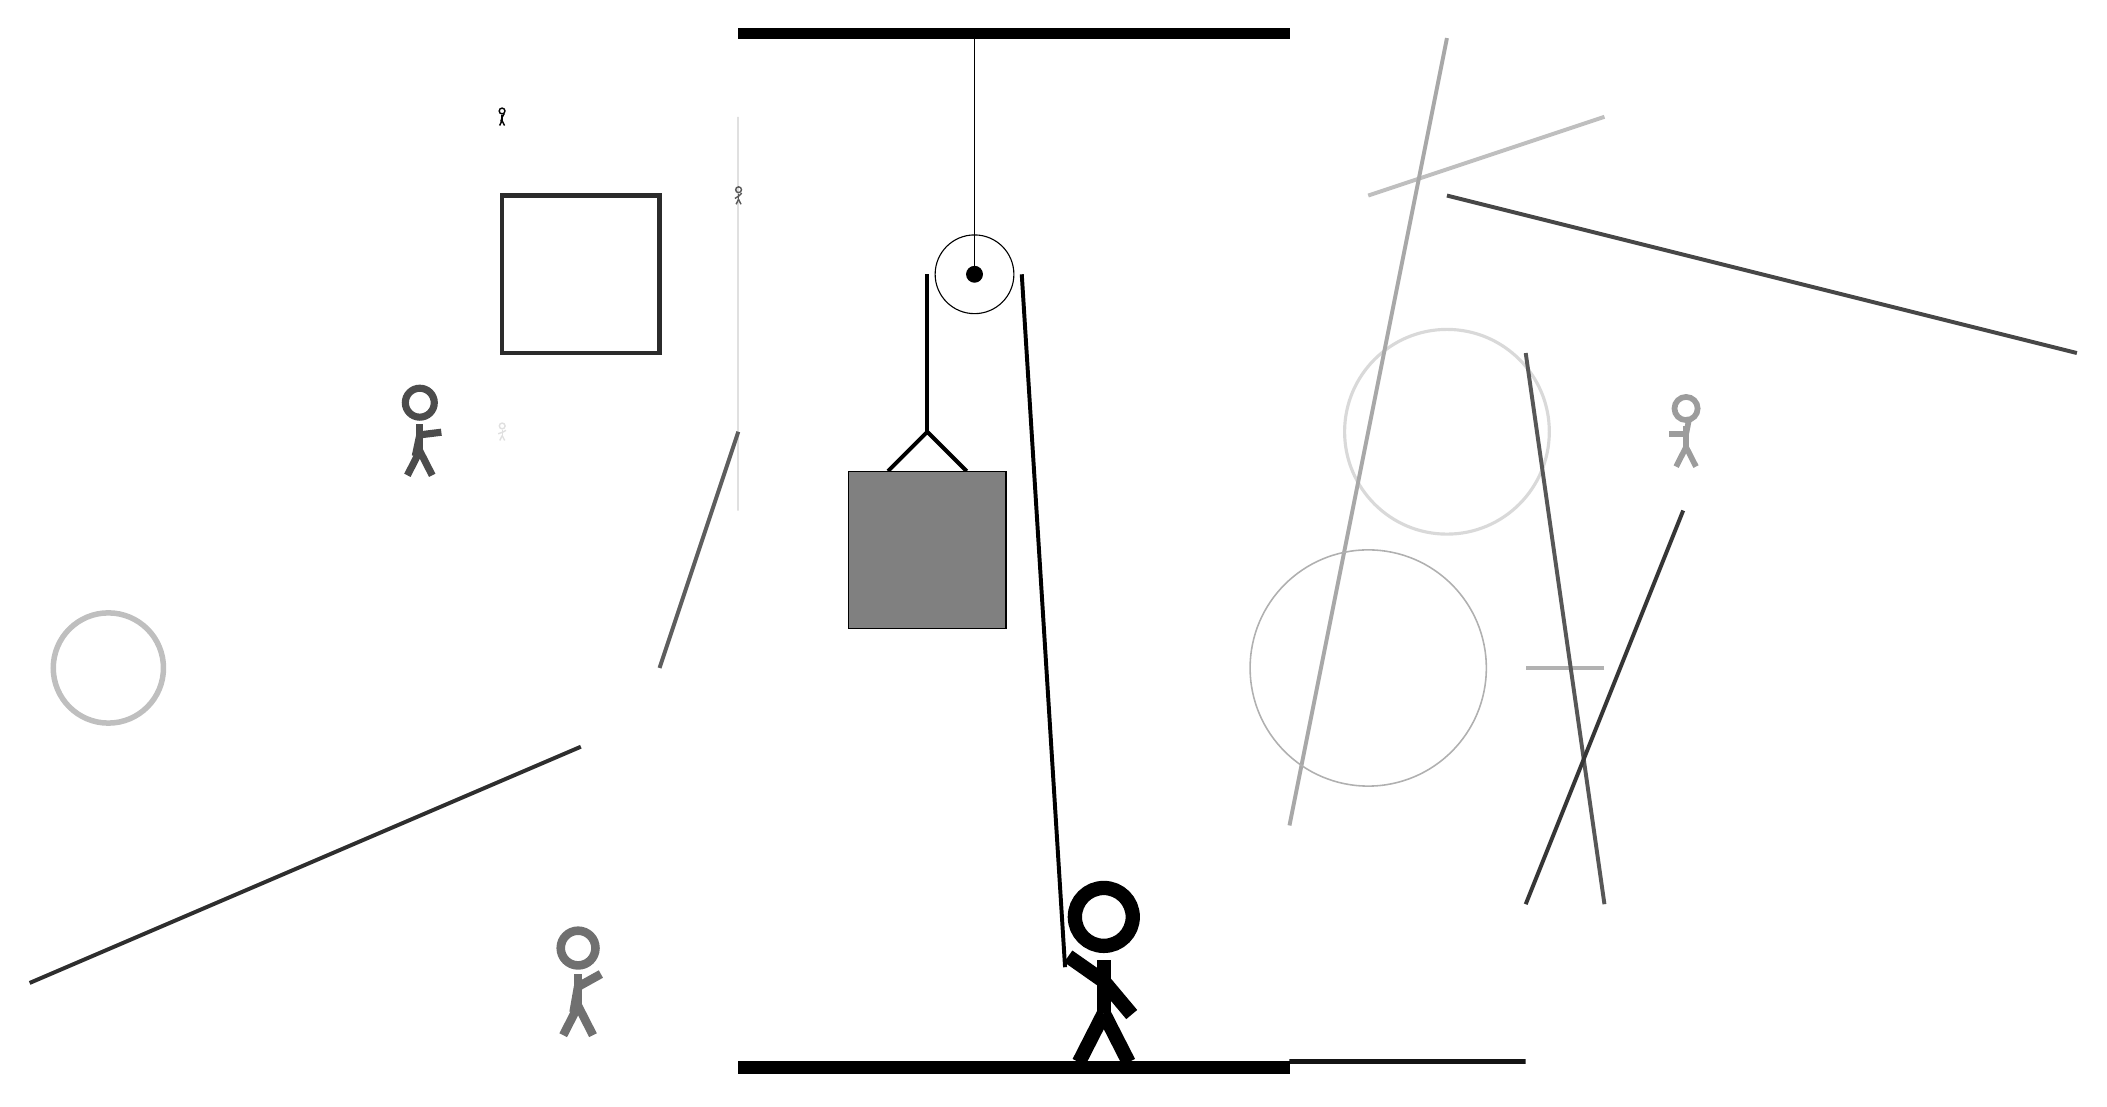
\begin{tikzpicture}
		%%%%% START %%%%%
		
		\draw[fill=black] (-2, 10) rectangle (5, 10.125);
		
		\draw (1, 7) circle (0.5);
		\draw[fill=black] (1, 7) circle (0.1);
		\draw (1, 10) -- (1, 7);
		
		\draw[line width=0.5mm] (-0.1, 4.5) -- (0.4, 5.0) -- (0.9, 4.5);
		\draw[fill=black!50] (-0.6, 4.5) rectangle (1.4, 2.5);
		
		\draw[line width=0.5mm] (0.4, 7) -- (0.4, 5.0);
		\centerarc[line width=0.5mm](1, 7)(0:180:0.6);
		\draw[line width=0.5mm](1.6, 7) -- (2.15, -1.8);
		
		\node at (2.6, -1.9) {\Strichmaxerl[10][-35][-50]};
		
		\draw[line width=0.3mm, color=black!12] (-2, 9) rectangle (-2, 4);
		
		\node[line width=0.3mm, color=black!70] at (-6, 5) {\Strichmaxerl[5][78][7]};
		\draw [line width=0.4mm, color=black!15](7, 5) circle (1.3);
		\draw[line width=0.5mm, color=black!30](9, 2) -- (8, 2);
		\draw[line width=0.6mm, color=black!92] (5, -3) rectangle (8, -3);
		\draw[line width=0.5mm, color=black!63](-2, 5) -- (-3, 2);
		\draw[line width=0.5mm, color=black!72](7, 8) -- (15, 6);
		
		\node[line width=0.2mm, color=black!12] at (-5, 5) {\Strichmaxerl[1][19][28]};
		\node[line width=0.5mm, color=black!65] at (-2, 8) {\Strichmaxerl[1][32][44]};
		\draw[line width=0.5mm, color=black!25](6, 8) -- (9, 9);
		\node[line width=0.2mm, color=black!98] at (-5, 9) {\Strichmaxerl[1][73][61]};
		\draw[line width=0.5mm, color=black!82](-4, 1) -- (-11, -2);
		\draw[line width=0.5mm, color=black!66](8, 6) -- (9, -1);
		
		\draw[line width=0.5mm, color=black!79](8, -1) -- (10, 4);
		\node[line width=0.3mm, color=black!39] at (10, 5) {\Strichmaxerl[4][0][79]};
		\draw[line width=0.5mm, color=black!34](5, 0) -- (7, 10);
		
		\draw [line width=0.2mm, color=black!31](6, 2) circle (1.5);
		
		\draw [line width=0.7mm, color=black!25](-10, 2) circle (0.7);
		\draw[line width=0.6mm, color=black!83] (-3, 6) rectangle (-5, 8);
		
		\node[line width=0.6mm, color=black!56] at (-4, -2) {\Strichmaxerl[6][80][29]};
		
		\draw[fill=black] (-2, -3) rectangle (5, -3.15);
		
		%%%%% END %%%%%
	\end{tikzpicture}
\end{document}